\documentclass[UTF8,a4paper,11pt,fontset=fandol]{ctexart}
\usepackage[margin=2.3cm]{geometry}
\usepackage{amsmath,amssymb,booktabs,graphicx,float,caption,needspace}
\usepackage[colorlinks=true,linkcolor=blue,citecolor=blue,urlcolor=blue]{hyperref}
\setlength{\parskip}{3pt}\clubpenalty=10000\widowpenalty=10000
\newcommand{\E}{\mathbb E}\newcommand{\N}{\mathcal N}\newcommand{\KL}{\operatorname{KL}}
\title{离散纵向数据的混合 GLMM 聚类\\\large 误差控制 MCEM、高斯变分近似与积分参照}
\author{课程大作业基础修订版}\date{2026 年 11 月 11 日}
\begin{document}\maketitle
\begin{abstract}
建立随机截距混合广义线性混合模型，用于二元、Poisson 和负二项纵向数据的个体聚类。实现独立重要性抽样 MCEM、高斯变分近似（GVA），以一维积分最大似然作参照。MCEM 最大化一个加权目标，并用独立样本评估更新增量误差；GVA 对 Poisson 使用解析期望。模拟覆盖轨迹分离、样本量、序列长度、簇数误设、方差及不规则时间。基准中GVA的平均ARI为0.885，积分参照为0.885；分离减半时GVA降至0.411。另在同一固定参数下比较变分近似、条件 MCMC 与积分。参数均为点估计，不将潜变量分布当作参数后验，不声称多起点获得全局最优。
\end{abstract}
\section{引言}
离散纵向数据兼有非高斯响应和个体内相关。混合 GLMM 将整条个体序列分配给一个潜在簇，以簇特异轨迹描述组间差异，以随机效应描述组内异质性。
Zeger--Karim\cite{zeger}讨论分层 GLMM 及条件随机效应抽样；McCulloch\cite{mcculloch}研究 MCEM、MCNR 和 SML 等似然算法；Booth--Hobert\cite{booth}利用独立抽样评估 MC 误差并增样。本文结合这些思想构造混合模型 MCEM，并用 Ormerod--Wand\cite{ormerod}的高斯变分近似作现代扩展。更新验证还参考 Caffo 等\cite{caffo}的上升思想，但下面的抽样、误差公式及预算为明确说明的本题适配，不是对其完整程序的复现。

\section{模型与似然}
个体 $i=1,\ldots,n$ 独立，时点为 $t_{ij}$，$j=1,\ldots,T_i$。设
\[
U_i\sim\operatorname{Cat}(\pi),\quad b_i\mid U_i=k\sim\N(0,D_k),\quad
\eta_{ijk}=\beta_{0k}+\beta_{1k}t_{ij}+b_i.
\]
给定 $(U_i,b_i)$ 后时间点条件独立。二元使用 logit link，计数使用 log link；负二项固定 size $a=5$，条件均值为 $\mu=e^\eta$、方差为 $\mu+\mu^2/a$。记 $\ell_{ik}(b;\beta_k)=\sum_j\log f(y_{ij};\eta_{ijk})$、$\omega_{ik}=1(U_i=k)$，则
\begin{align}
\log L_c(\Omega)&=\sum_{ik}\omega_{ik}\{\log\pi_k+\log\phi(b_i;0,D_k)+\ell_{ik}(b_i;\beta_k)\},\\
L(\Omega;Y)&=\prod_i\sum_k\pi_k A_{ik},\quad
A_{ik}=\int e^{\ell_{ik}(b;\beta_k)}\phi(b;0,D_k)\,db.
\end{align}
未观测时点不求和，未被选择的簇不需额外的随机效应。模型不含随机斜率或额外时间相关结构。

\section{方法}
\subsection{MCEM 的 E 步与单目标 M 步}
以 $(U,b)$ 为缺失数据，将 McCulloch 的 MCEM 分解加入类别责任度。在旧参数 $\Omega^r$ 下，
\[
\tau_{ik}=\frac{\pi_k A_{ik}}{\sum_h\pi_h A_{ih}},\quad
h_{ik}(b)=p(b_i\mid Y_i,U_i=k;\Omega^r)\propto e^{\ell_{ik}(b;\beta_k^r)}\phi(b;0,D_k^r).
\]
这与 Zeger--Karim 的条件随机效应计算直接相连；其全贝叶斯方案另抽样参数，本文不做参数 Gibbs。该文主要用拒绝抽样处理非标准条件分布，不能把所有步骤都写成 MH。
沿用 Booth--Hobert 的独立 $t$ 重要性抽样思想，以带回溯的 Newton 法求条件众数 $\widehat b_{ik}$ 和逆曲率 $V_{ik}=\{-\ell''_{ik}(\widehat b_{ik})+1/D_k^r\}^{-1}$。最多80轮，位移容差 $10^{-9}$，核对得分残差。每个 $(i,k)$ 独立抽 $M$ 个 $t_5(\widehat b_{ik},s_{ik}^2)$，scale平方为 $s_{ik}^2=3V_{ik}/5$，使方差为 $V_{ik}$。令
\[
v_{ikm}=\frac{\pi_k^r e^{\ell_{ik}(b_{ikm};\beta_k^r)}\phi(b_{ikm};0,D_k^r)}{q_{ik}(b_{ikm})},\quad
a_{ikm}=\frac{v_{ikm}}{\sum_{h,l}v_{ihl}}.
\]
于是 $\widehat\tau_{ik}=\sum_m a_{ikm}$，$w_{ikm}=a_{ikm}/\widehat\tau_{ik}$，层内有效样本量为 $\operatorname{ESS}_{ik}=1/\sum_mw_{ikm}^2$，实际 MC 目标为
\[
\widehat Q=\sum_{ikm}a_{ikm}\{\log\pi_k+\log\phi(b_{ikm};0,D_k)+\ell_{ik}(b_{ikm};\beta_k)\}.
\]
自归一化比率有有限样本偏差，不能称为无偏 log 似然。令 $N_k=\sum_i\widehat\tau_{ik}$，则
\[
\pi_k^+=N_k/n,\quad D_k^+=\frac{\sum_{im}a_{ikm}b_{ikm}^2}{N_k},\quad
\beta_k^+=\arg\max_\beta\sum_{im}a_{ikm}\ell_{ik}(b_{ikm};\beta).
\]
方差投影到允许区间，固定效应用解析梯度的 L-BFGS-B，最多80次；各簇目标除以 $N_k$，函数容差 $10^{-12}$、梯度目标 $10^{-7}$。检查同一个 $\widehat Q$ 不减并记录该尺度的投影梯度；内部仅完成目标改善时属于广义 M 步，不声称精确极大化。修订版不平均两次 M 步的参数。

\subsection{独立验证、MC 标准误与停止}
候选 $\Omega^+$ 由训练样本得到，再在 $\Omega^r$ 下独立抽验证样本。设
\[
d_{ikm}=\log L_{ci}(\Omega^+;k,b_{ikm})-\log L_{ci}(\Omega^r;k,b_{ikm}),\quad
\widehat\Delta_i=\sum_{km}a_{ikm}d_{ikm},\quad z_{ikm}=a_{ikm}(d_{ikm}-\widehat\Delta_i).
\]
将各层独立样本均值的方差经比率的一阶导数传播，得到分层自归一化 IS 的 delta 方法估计
\begin{equation}
\widehat{\operatorname{Var}}_{MC}(\widehat\Delta)
=\sum_{ik}\frac{M}{M-1}\sum_m(z_{ikm}-\bar z_{ik})^2,\quad
\widehat\Delta=\sum_i\widehat\Delta_i.
\end{equation}
用个体联合均值 $\widehat\Delta_i$ 居中，故包含责任度归一化误差；只按每簇条件均值居中会遗漏它。独立验证使候选在误差计算中可视为固定。
令 $s_\Delta$ 为标准误，$L=\widehat\Delta-1.96s_\Delta$、$H=\widehat\Delta+1.96s_\Delta$。$L>0$ 则接受，否则保持旧参数。不能确定上升且未满足精度时增样；ESS比例第10百分位小于0.4也增样。每层 $M$ 从128加倍至最多8192。
连续三轮满足 $H/n<5\times10^{-5}$、$s_\Delta/n<2\times10^{-5}$、缩放位移 $\max_j|\theta_j^+-\theta_j^r|/(1+|\theta_j^r|)<0.01$、M步投影梯度 $<10^{-4}$ 则停止。$\theta$ 为固定效应、log方差、混合比例logits。最多250轮；样本上限仍不能决策则标记预算不足，不算收敛。
正态区间是独立 IS 的渐近点态近似，不消除有限样本比率偏差，多轮查看也不是整个算法的95\%上升保证。不直接继承原文完整收敛定理；用经验重复核对 MCSE，以积分估计核对最终差距。

\subsection{高斯变分近似：现代扩展}
取 $q(U_i=k,b_i)=r_{ik}\N(b_i;m_{ik},s_{ik}^2)$，个体间分解，保留标签与随机效应的条件依赖。证据下界为
\begin{align}
\mathcal L(q,\Omega)&=\sum_{ik}r_{ik}\{\log\pi_k-\log r_{ik}+F_{ik}\},\\
F_{ik}&=\E_q\ell_{ik}(b)-\frac12\left\{\frac{m_{ik}^2+s_{ik}^2}{D_k}-1+\log\frac{D_k}{s_{ik}^2}\right\}.
\end{align}
固定参数时 $\log L-\mathcal L=\KL(q\|p(U,b\mid Y;\Omega))\geq0$。每个局部 $(m,s)$ 最大化 $F$，然后 $r_{ik}\propto\pi_ke^{F_{ik}}$。以 $b=m+sZ$、$Z\sim\N(0,1)$，
\[
F_m=\E\ell'(m+sZ)-m/D,\quad F_s=\E[Z\ell'(m+sZ)]+1/s-s/D.
\]
若 $H=-\ell''\geq0$，负 Hessian 为
\[
\E\left[H\begin{pmatrix}1&Z\\Z&Z^2\end{pmatrix}\right]
+\operatorname{diag}(1/D,1/D+1/s^2),
\]
故本题三类正确似然的局部目标在 $s>0$ 严格凹。用独立二维 Newton 加回溯，保持 $s$ 正且目标不减；最多100轮，局部梯度目标 $10^{-7}$，最终残差另行记录。
Poisson 使用解析式
\[
\E_q\ell_{ik}=\sum_j\{y_{ij}(x_{ij}^\top\beta_k+m_{ik})
-e^{x_{ij}^\top\beta_k+m_{ik}+s_{ik}^2/2}-\log(y_{ij}!)\}.
\]
其余响应使用31点正权 GH，$\E H(Z)\approx\pi^{-1/2}\sum_l a_lH(\sqrt2x_l)$。有限积分只是近似目标，不能无条件称其仍为精确似然的严格下界。
外层最大化局部变分参数优化后的剖面 ELBO。包络梯度为
\begin{align}
\partial_{\beta_k}\mathcal L&=\sum_i r_{ik}\E_q\partial_{\beta_k}\ell_{ik},\\
\partial_{\log D_k}\mathcal L&=\tfrac12\sum_i r_{ik}\{(m_{ik}^2+s_{ik}^2)/D_k-1\},\\
\partial_{\alpha_k}\mathcal L&=\sum_i r_{ik}-n\pi_k,\quad \alpha_k=\log(\pi_k/\pi_K),\ k<K.
\end{align}
以每个体平均负目标作 L-BFGS-B，函数容差 $10^{-12}$、梯度目标 $2\times10^{-6}$、最多300轮；最终投影梯度 $<10^{-4}$ 且局部残差 $<10^{-5}$ 才标记数值收敛。

\subsection{积分参照、初始化与实现}
随机截距一维，使用61点自适应 GH 计算 $A_{ik}$：以条件众数和逆曲率构造正态密度 $q_N$，求 $\E_{q_N}[e^{\ell_{ik}}\phi/q_N]$。最大化观测 log 似然，Fisher 恒等式给出其梯度，即把上面的变分期望换成条件积分期望。优化设置同 GVA，最后用101点复核。称为数值积分 ML（QML）参照，不称为全局真值。
单观测对 $\eta$ 的得分为 $y-p$、$y-e^\eta$、$y-(y+5)p_a$，负二阶导数为 $p(1-p)$、$e^\eta$、$(y+5)p_a(1-p_a)$；$p=\operatorname{logit}^{-1}(\eta)$、$p_a=e^\eta/(5+e^\eta)$。对 $\beta$ 乘 $(1,t)^\top$ 后求和。Poisson 还利用随机截距充分统计量降低重复计算，不截断 $e^\eta$ 改变模型，机器溢出的零权重尾部按数值零处理。

每拟合3起点：个体响应均值和时间斜率构成特征，$\widehat d_i=\sum_j(t_{ij}-\bar t_i)y_{ij}/\max\{\sum_j(t_{ij}-\bar t_i)^2,10^{-6}\}$。二元平滑均值为 $p_i=(\sum_jy_{ij}+0.5)/(T_i+1)$，特征为 $\{\operatorname{logit}(p_i),\widehat d_i/[p_i(1-p_i)]\}$；计数为 $\{\log(\bar y_i+0.1),\widehat d_i/(\bar y_i+0.1)\}$。斜率特征截在 $[-4,4]$，各特征加标准差0.08的正态扰动，用 k-means++ 加30轮聚类初始化：中心作 $\beta$，组内人数比例作 $\pi$，各方差初值0.5，不用真实标签。
$\beta\in[-8,8]$、$D_k\in[0.005,5]$；QML/GVA logits限 $[-16,16]$，MCEM 遇到 $\pi_k<10^{-12}$ 报告数值空分量。MCEM/QML 按最终积分似然选起点，GVA 按 ELBO 选；最大责任度给聚类。匹配真实标签仅用于评价，不证明识别性或全局最优。

\subsection{同目标条件 MCMC}
固定同一 QML 参数，目标为 $p(U,b\mid Y;\widehat\Omega)$，不抽样参数。最初分开更新标签和随机效应的Gibbs/MH检查中，Poisson接受率约0.877，但最大split诊断约36，链未混合；该输出保留，不作精度真值。标签与随机截距的强依赖需要联合跨模式更新。正式比较使用标准联合独立MH：由 $g_i(h,b^*)=\pi_h q_{ih}(b^*)$ 提议新标签和随机效应。若当前标签为 $k$，目标与提议中的混合比例抵消后，接受率为
\[
\min\left\{1,\frac{e^{\ell_{ih}(b^*)}\phi(b^*;0,D_h)q_{ik}(b_i)}{e^{\ell_{ik}(b_i)}\phi(b_i;0,D_k)q_{ih}(b^*)}\right\}.
\]
$q_{ih}$ 沿用上述基于条件众数和曲率的$t_5$提议，在固定参数下不再调整。三个响应场景第一次重复各取前30个体，4链各2000次预热、8000次保留。起始标签为0、1、2、0，$b$ 为相应条件众数。保存全部样本；报告经典 split $\widehat R$（非秩标准化）和长度100的批均值 MCSE；均值、方差、责任度与101点积分比较。有限链不是无误差的后验真值，也不能用来声称参数后验区间的准确性。

\section{模拟研究}
\subsection{设计与评价}
基准为 $n=300,T=20$，等距时间 $[-1,1]$，真值和拟合 $K=3$，$\pi=(0.5,0.3,0.2)$、$D_k=0.5$，二元响应；$\beta_k$ 为 $(-1.5,-1.8),(0.5,1.8),(1.5,-1.8)$。另保留作业建议 $(-1.5,0.2),(0.5,-0.2),(1,0.3)$ 作为困难场景。
14场景为：基准；$\beta_k$ 向三簇均值收缩一半；作业建议参数；$n=100,1000$；$T=10,50$；拟合 $K=2,4$；$D_k=0.1,1.5$；Poisson；负二项；不规则时间。最后一项先生成每人20个排序的均匀时间，再独立取 $T_i\in\{10,\ldots,20\}$ 并保留前 $T_i$ 个，因此部分人的观测偏向早期，不声称均匀覆盖区间。
GVA/QML 各场景5次重复；MCEM 在基准二元、Poisson、负二项各5次，每次3起点，共70份不同数据、155次拟合。不声称每个方法在每个场景均运行。数据种子 $20261110+10000s+r$，场景 $s=0,\ldots,13$ 按上段顺序，重复 $r=0,\ldots,4$；拟合种子加200000，起点再加 $1009h$，MC流另加73。MCMC种子为 $20261110+900000+f$，$f=0,1,2$ 为二元、Poisson、负二项。
服务器可用16个逻辑CPU、内存限额约80 GiB，使用8个并行拟合进程，每进程数值库单线程；Python 3.11.4、NumPy 2.4.2、SciPy 1.16.3、Matplotlib 3.10.8。源码、配置、逐起点记录、全部保留MCMC样本及SHA256清单在本地保存。

ARI 对标签置换不变并校正随机一致性；错分率用最优一对一匹配。正确 $K$ 时按固定效应距离匹配，分别计算固定效应、方差、比例的 RMSE；误设 $K$ 不强行一一比较参数。表中为重复均值，ARI另列样本标准差；5次重复仍只支持初步观察。全部预算不足或未收敛结果保留。
\subsection{结果}
\begin{table}[H]\centering\small
\caption{全部14场景的5次重复。ARI为均值$\pm$标准差；RMSE为GVA跨重复均值，误设$K$不比较参数。收敛数按QML/GVA，分母各为5。}
\begin{tabular}{lcccccc}\toprule
场景 & ARI(QML) & ARI(GVA) & $\beta$ RMSE & $D$ RMSE & $\pi$ RMSE & 收敛\\\midrule
基准 & 0.885$\pm$0.038 & 0.885$\pm$0.038 & 0.133 & 0.181 & 0.033 & 5/5 \\
分离减半 & 0.412$\pm$0.082 & 0.411$\pm$0.083 & 0.439 & 0.282 & 0.130 & 5/5 \\
作业建议参数 & 0.411$\pm$0.121 & 0.363$\pm$0.118 & 0.891 & 0.552 & 0.249 & 5/5 \\
$n=100$ & 0.806$\pm$0.101 & 0.806$\pm$0.101 & 0.301 & 0.251 & 0.050 & 5/5 \\
$n=1000$ & 0.882$\pm$0.021 & 0.882$\pm$0.020 & 0.075 & 0.120 & 0.025 & 5/5 \\
$T=10$ & 0.734$\pm$0.125 & 0.754$\pm$0.090 & 0.303 & 0.430 & 0.053 & 5/5 \\
$T=50$ & 0.939$\pm$0.032 & 0.939$\pm$0.032 & 0.088 & 0.121 & 0.026 & 5/5 \\
$K=2$ & 0.593$\pm$0.038 & 0.593$\pm$0.038 & -- & -- & -- & 5/5 \\
$K=4$ & 0.820$\pm$0.038 & 0.822$\pm$0.037 & -- & -- & -- & 5/5 \\
$D=0.1$ & 0.970$\pm$0.013 & 0.970$\pm$0.013 & 0.094 & 0.051 & 0.022 & 5/5 \\
$D=1.5$ & 0.654$\pm$0.110 & 0.662$\pm$0.114 & 0.419 & 0.584 & 0.107 & 5/5 \\
Poisson & 0.959$\pm$0.016 & 0.955$\pm$0.014 & 0.064 & 0.120 & 0.030 & 5/5 \\
负二项 & 0.973$\pm$0.014 & 0.975$\pm$0.011 & 0.073 & 0.071 & 0.029 & 5/5 \\
不规则时间 & 0.609$\pm$0.047 & 0.616$\pm$0.042 & 0.249 & 0.455 & 0.041 & 5/5 \\
\bottomrule\end{tabular}\end{table}

\begin{table}[H]\centering\small
\caption{三类响应的同数据比较。各格为5次均值；耗时为三起点总墙钟秒数。原停止按第3节原算法规则，新增似然口径另表核验。$\Delta\ell/n=(\ell_{\mathrm{QML}}-\ell_{\mathrm{fit}})/n$，fit表示对应方法，可因不同局部解出现负值，不是KL散度。}
\begin{tabular}{llcccccc}\toprule
响应 & 方法 & ARI & 错分率 & $\beta$ RMSE & 秒 & 原停止/5 & $\Delta\ell/n$\\\midrule
基准 & QML & 0.885$\pm$0.038 & 0.042 & 0.133 & 24.3 & 5 & 0.00000 \\
基准 & GVA & 0.885$\pm$0.038 & 0.042 & 0.133 & 40.2 & 5 & 0.00000 \\
基准 & MCEM & 0.899$\pm$0.020 & 0.037 & 0.126 & 728.6 & 5 & 0.00027 \\
Poisson & QML & 0.959$\pm$0.016 & 0.014 & 0.063 & 7.6 & 5 & 0.00000 \\
Poisson & GVA & 0.955$\pm$0.014 & 0.015 & 0.064 & 8.2 & 5 & 0.00001 \\
Poisson & MCEM & 0.956$\pm$0.022 & 0.015 & 0.090 & 373.3 & 5 & 0.00407 \\
负二项 & QML & 0.973$\pm$0.014 & 0.009 & 0.073 & 35.8 & 5 & 0.00000 \\
负二项 & GVA & 0.975$\pm$0.011 & 0.009 & 0.073 & 71.7 & 5 & 0.00001 \\
负二项 & MCEM & 0.969$\pm$0.008 & 0.011 & 0.094 & 2779.9 & 5 & 0.00092 \\
\bottomrule\end{tabular}\end{table}

\Needspace{4\baselineskip}基准GVA的平均ARI为0.885、错分率0.042；分离减半和作业建议参数时ARI为0.411、0.363。全部155次原拟合中，155次满足各自原停止标准；新增似然检查见补充表，内部求解器状态和参数边界另行记录。各因素的实测结果见表，不从5次重复推断普遍优势。不同目标的差异、同一目标的积分误差和参数恢复误差分别评价。Poisson场景GVA三起点平均耗时8.2秒、收敛5/5；其解析期望与剖面优化的实现不再采用旧版高维局部数值优化，但新旧硬件/容差不同，不能直接用旧耗时计算加速比。MCEM所选解的每个体观测目标投影得分最大范数范围为0.001222至0.05756；小Q增量并不直接保证观测得分为零，表中的剩余似然差也须同时查看。MCEM在二元、Poisson、负二项下的方差参数RMSE依次为0.145、0.112、0.078，混合比例RMSE依次为0.029、0.026、0.034。另有4次所选起点记录过内部求解器非成功状态，与外层停止标记分开保存。有28次所选解触及预设方差或固定效应边界，参数解释受约束影响。样本量100至1000时，GVA固定效应RMSE由0.301变为0.075；序列10至50次时ARI由0.754变为0.939。方差0.1与1.5的ARI为0.970/0.662；拟合2簇与4簇为0.593/0.822，不规则时间为0.616。基准5份数据中，每个体终目标的三起点极差最大值，QML、GVA、MCEM依次为1.19e-10、4.993e-11、0.0003116；各方法按自己的目标衡量，MCEM差异还含MC波动，不能据此证明全局最优。
\begin{figure}[H]\centering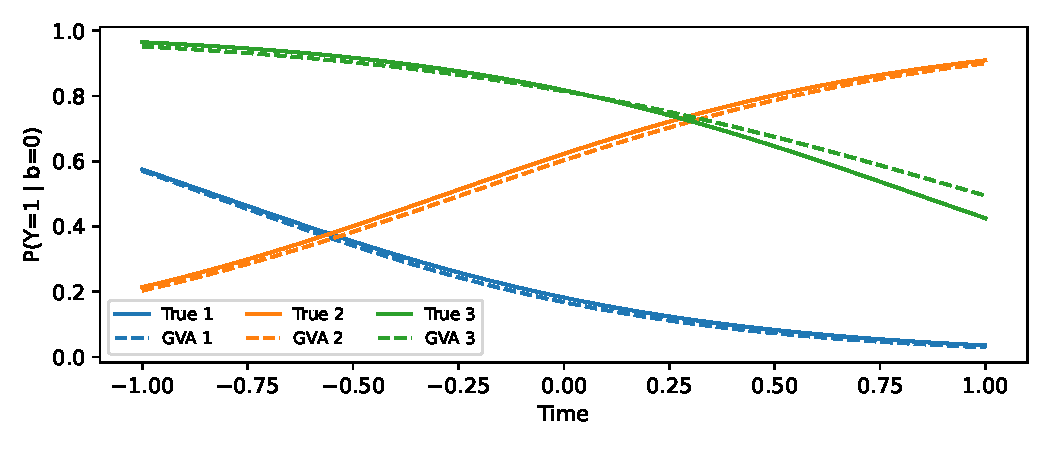
\includegraphics[width=.85\linewidth]{figures/trajectories.pdf}\caption{基准第一次重复的真实与 GVA 拟合条件轨迹，随机截距取0，不是总体平均轨迹。}\end{figure}
\begin{figure}[H]\centering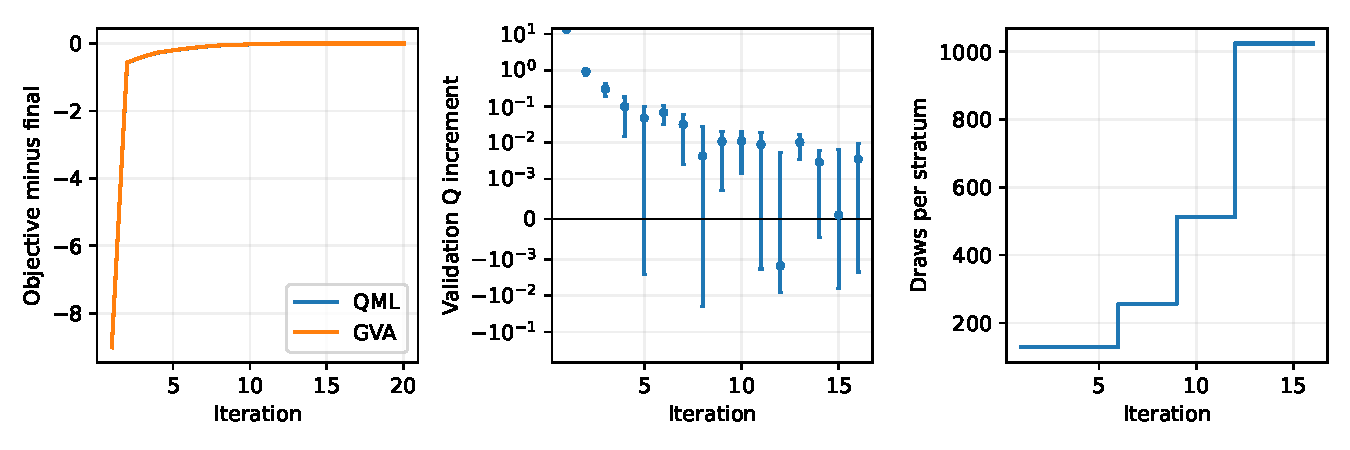
\includegraphics[width=\linewidth]{figures/diagnostics.pdf}\caption{基准第一次重复所选起点：各自目标相对终值、MCEM 验证增量区间、每层抽样量。目标曲线不用于跨目标直接比较。}\end{figure}
\subsection{数值与条件分布核验}
剖面梯度与中心差分核对；Poisson 解析期望与高阶积分核对，并检查 $\eta>50$ 的梯度一致性。MCSE 与80次独立抽样的经验标准差对照，细节见 \texttt{qa/validation.json}。
\begin{table}[H]\centering\small
\caption{同一固定QML参数下，30个体条件分布的核验。误差对101点积分计算；成对数值为MCMC/GVA。方差比为各个体边缘$b_i$方差之和相对于积分的比。}
\begin{tabular}{lccccc}\toprule
响应 & MH接受率 & 最大split $\widehat R$ & 均值RMSE & 责任度RMSE & 方差比\\\midrule
基准 & 0.365 & 1.0021 & 0.0083/0.0002 & 0.0026/0.0001 & 0.995/0.997 \\
Poisson & 0.357 & 1.0038 & 0.0045/0.0002 & 0.0011/0.0000 & 1.002/0.986 \\
负二项 & 0.354 & 1.0016 & 0.0047/0.0002 & 0.0007/0.0000 & 0.996/0.990 \\
\bottomrule\end{tabular}\end{table}
在小规模80次独立IS检验中，经验标准差与delta方法预测标准差之比分别为1.025、1.040、1.013。这是误差公式的有限验证，不是所有场景的覆盖率证明。全部所选参数的61与101点积分log似然最大差为1.55e-11。全部MCEM起点实际生成7,439,846,400个提议值；若对相同的已发生迭代都固定使用每层8192，则为45,608,140,800个，前者占0.163。这仅比较相同迭代数的抽样量，不是固定样本算法达到同等精度的时间比。14场景第一次重复的GVA，以61点替换31点后重新求局部最优，剖面ELBO最大绝对差为1.82e-12。条件MCMC的个体均值批均值MCSE（对30人再平均）依次为0.0069、0.0032、0.0048。本例GVA与积分的差异很小，有限MCMC仍有抽样误差；这不表示变分推断普遍比充分计算的MCMC更准确。这些结果针对固定参数的潜变量目标，未构造全贝叶斯参数区间。
\begin{figure}[H]\centering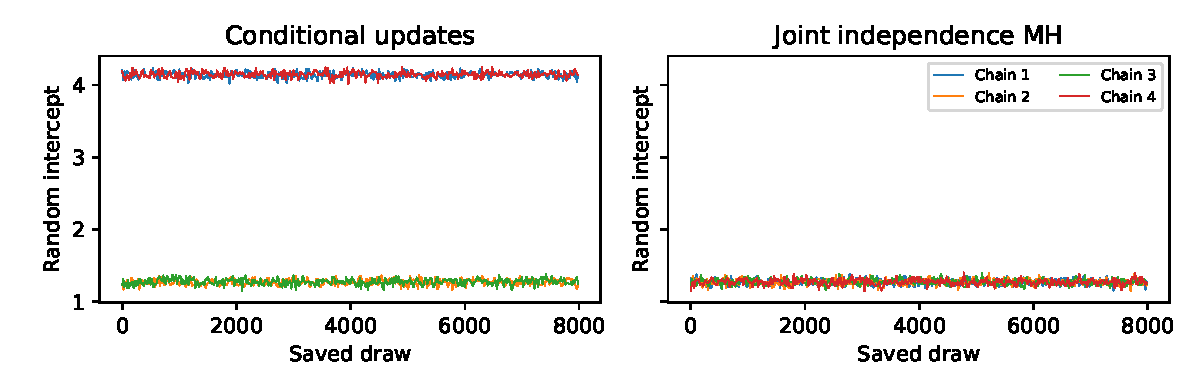
\includegraphics[width=.9\linewidth]{figures/mcmc_trace.pdf}\caption{Poisson同一参数下的链。选择原分开更新中split诊断最大的个体作示例；右图用标准联合独立MH跨越标签--随机截距的联合模式。轨迹每20次显示一点，诊断使用全部保留样本。}\end{figure}

\section{讨论}
MCEM 继承缺失数据分解和独立重要性抽样；增量误差包括责任度归一化。GVA 为现代扩展，利用高斯族及 Poisson 解析结构。其误差包含变分族限制、积分与优化误差；同一参数的 MCMC/积分比较只检验潜变量近似，不能验证参数后验区间。单个GLMM中已有的GVA一致性结果也不能直接当作本混合模型的一致性证明，本文仅作数值验证。

局部变分目标严格凹不代表整体混合目标凹，3起点不能排除局部最优。轨迹重叠和较大随机效应方差使成员难区分，真实标签匹配只校正编号。$K$ 过小合并簇、过大可能拆分簇；本文不做数据驱动选 $K$。点估计没有参数先验敏感性实验；随机效应分布是模型假设，不是参数先验。若做全贝叶斯推断，应使用适当可积先验，并让 VB 与 MCMC 针对同一后验比较。

一维 GH 提供便宜参照；更多随机效应会带来积分维数增长，IS也可能退化。样本存储约 $O(nKM)$，似然约 $O(nKTM)$，Poisson可用充分统计量降低重复计算。只比较到 $n=1000$，不声称解决大规模计算。耗时含全部起点与诊断，云端进程竞争及不同停止标准影响墙钟时间，不能将速度比解释为同等精度下的普遍结论。
本次三个响应场景中，GVA的实测耗时均小于MCEM，而一维QML又均快于GVA；因此本题的低维积分结构本身有计算优势，不能仅因采用现代扩展就预设其最快。

正态随机效应和给定 $(U,b)$ 后时间独立是假设，未对其误设额外模拟。MCEM区间是渐近点态近似，预算可能不足；积分法和 GVA 也保留非成功状态。数值稳定不是全局最优或统计识别性的证明。

模拟设计中，原建议二元参数较难区分，故同时保留困难场景和更分离的基准。随机截距本身可使边缘计数过度离散，负二项另增条件过度离散；固定 size=5 不代表解决未知离散度估计。不同族相同线性预测器不意味着相同信息量。后续宜先增加重复并研究困难场景，避免任意堆叠模型。

\begin{thebibliography}{9}
\bibitem{zeger} Zeger, S. L. and Karim, M. R. (1991). Generalized linear models with random effects: a Gibbs sampling approach. \emph{JASA}, 86, 79--86.
\bibitem{mcculloch} McCulloch, C. E. (1997). Maximum likelihood algorithms for generalized linear mixed models. \emph{JASA}, 92, 162--170.
\bibitem{booth} Booth, J. G. and Hobert, J. P. (1999). Maximizing generalized linear mixed model likelihoods with an automated Monte Carlo EM algorithm. \emph{JRSS-B}, 61, 265--285.
\bibitem{ormerod} Ormerod, J. T. and Wand, M. P. (2012). Gaussian variational approximate inference for generalized linear mixed models. \emph{JCGS}, 21, 2--17. \href{https://doi.org/10.1198/jcgs.2011.09118}{doi:10.1198/jcgs.2011.09118}.
\bibitem{caffo} Caffo, B. S., Jank, W. and Jones, G. L. (2005). Ascent-based Monte Carlo expectation--maximization. \emph{JRSS-B}, 67, 235--251. \href{https://doi.org/10.1111/j.1467-9868.2005.00499.x}{doi:10.1111/j.1467-9868.2005.00499.x}.
\end{thebibliography}\end{document}
